\documentclass[border=0.5cm]{standalone}
\usepackage{tikz}
\usetikzlibrary{arrows, arrows.meta, tikzmark}

\tikzset{    
    disk/.style={ thick },
    traj/.style={ thin, dotted, -Latex },
    point/.style={ color=black, circle, scale=0.3, fill },
    partition/.style={ right, scale=0.75 }
}

\definecolor{light-gray}{gray}{0.9}

\def\xMin{0}
\def\xMax{9}
\def\yMin{0}
\def\yMax{5}
\def\R{0.9}
\def\gap{0.2}
\def\rowspace{0.25}

\begin{document}
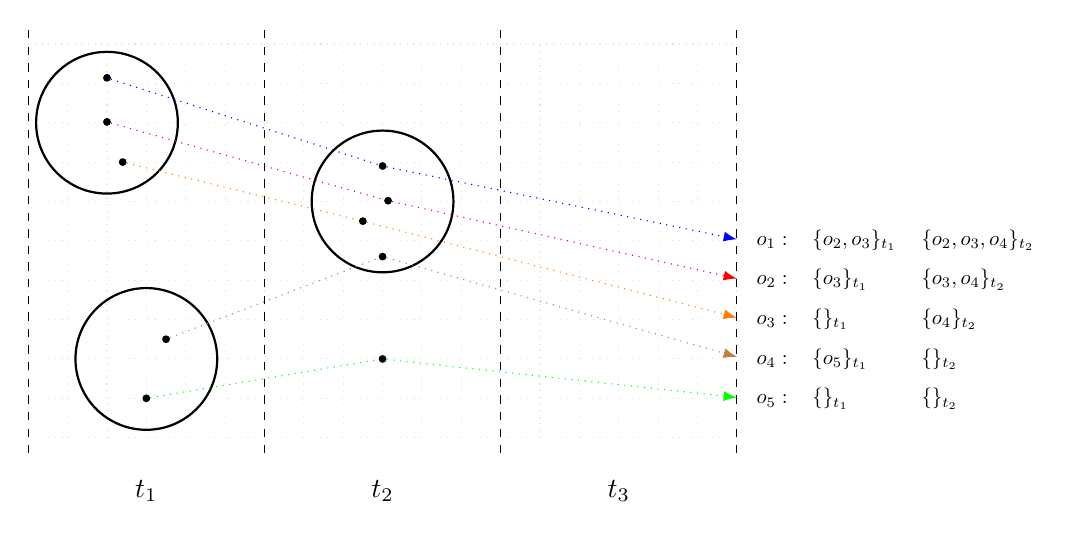
\begin{tikzpicture}
    \draw[color=light-gray, style=dotted, step=0.5] (0,0) grid (9,5);
    \draw[dashed] (0,\yMin-\gap) -- (0,\yMax+\gap);
    \draw[disk] (1,4) circle (\R);
    \draw[disk] (1.5,1) circle (\R);
    \draw[dashed] (3,\yMin-\gap) -- (3,\yMax+\gap);
    \draw[disk] (4.5,3) circle (\R);
    \draw[dashed] (6,\yMin-\gap) -- (6,\yMax+\gap);
    %\draw[disk] (7.5,1.75) circle (\R);
    \draw[dashed] (9,\yMin-\gap) -- (9,\yMax+\gap);
    \node[very thick, below] at (1.5,\yMin-\gap-\gap) {$t_1$};
    \node[very thick, below] at (4.5,\yMin-\gap-\gap) {$t_2$};
    \node[very thick, below] at (7.5,\yMin-\gap-\gap) {$t_3$};
    
    \node[partition] (partitions) at (\xMax, 1.5) {
        \begin{tabular}{l l l}
            $o_1: $ & $\{o_2, o_3\}_{t_1}$  & $\{o_2, o_3, o_4\}_{t_2}$ \\[\rowspace cm]
            $o_2: $ & $ \{o_3\}_{t_1}$      & $\{o_3, o_4\}_{t_2}$      \\[\rowspace cm]
            $o_3: $ & $ \{ \}_{t_1}$        & $\{o_4\}_{t_2}$           \\[\rowspace cm]
            $o_4: $ & $ \{o_5 \}_{t_1}$     & $\{\}_{t_2}$              \\[\rowspace cm]
            $o_5: $ & $ \{ \}_{t_1}$        & $\{\}_{t_2}$              \\
        \end{tabular}
    };

    % Trajectories
    \node[point] (A1) at (1, 4.57) {};
    \node[point] (A2) at (4.5, 3.45) {};
    %\node[point] (A3) at (7.5, 2.15) {};
    \node[partition] (A) at (\xMax, 2.5) {};
    \draw[traj, blue]  (A1) -- (A2) -- (A); 

    \node[point] (B1) at (1, 4.01) {};
    \node[point] (B2) at (4.57, 3.01) {};
    %\node[point] (B3) at (7.5, 1.8) {};
    \node[partition] (B) at (\xMax, 2) {};
    \draw[traj, red]  (B1) -- (B2) -- (B);

    \node[point] (C1) at (1.2, 3.5) {};
    \node[point] (C2) at (4.25, 2.75) {};
    %\node[point] (C3) at (7.6, 1.5) {};
    \node[partition] (C) at (\xMax, 1.5) {};
    \draw[traj, orange]  (C1) -- (C2) -- (C);

    \node[point] (D1) at (1.75, 1.25) {};
    \node[point] (D2) at (4.5, 2.3) {};
    %\node[point] (D3) at (7.25, 1.25) {};
    \node[partition] (D) at (\xMax, 1) {};
    \draw[traj, brown]  (D1) -- (D2) -- (D);

    \node[point] (E1) at (1.5, 0.5) {};
    \node[point] (E2) at (4.5, 1.0) {};
    %\node[point] (E3) at (8.0, 0.5) {};
    \node[partition] (E) at (\xMax, 0.5) {};
    \draw[traj, green]  (E1) -- (E2) -- (E);

    %%%%%
    %\foreach \i in {\xMin,...,\xMax} { \node[very thin,gray,below,scale=0.5] at (\i,\yMin) {$\i$}; }
    %\foreach \i in {\yMin,...,\yMax} { \node[very thin,gray,left ,scale=0.5] at (\xMin,\i) {$\i$}; }    
    %%%%%
\end{tikzpicture}
\end{document}
